\documentclass{article}
\usepackage{hyperref}
\usepackage{listings}
\usepackage{color}
\usepackage{xcolor}
\usepackage{geometry}
\usepackage{graphicx}
\usepackage{amsmath}
\usepackage{caption}
\usepackage{subcaption}
\geometry{margin=1in}
\pdfminorversion=6

\newcommand\TODO[1]{\textcolor{red}{TODO: #1}}

\newcommand\header[2]{
    \begin{center}
        {\large
        UCSD CSE 168 Assignment #1: \\
        \vspace{0.3cm}
        \Large
        #2}
    \end{center}
}

\definecolor{dkgreen}{rgb}{0,0.6,0}
\definecolor{gray}{rgb}{0.5,0.5,0.5}
\definecolor{mauve}{rgb}{0.58,0,0.82}
\lstset{frame=tb,
        aboveskip=3mm,
        belowskip=3mm,
        showstringspaces=false,
        columns=flexible,
        basicstyle={\small\ttfamily},
        numbers=none,
        numberstyle=\tiny\color{gray},
        keywordstyle=\color{blue},
        commentstyle=\color{dkgreen},
        stringstyle=\color{mauve},
        breaklines=true,
        breakatwhitespace=true,
        tabsize=2
}

\hypersetup{colorlinks=true}

\usepackage{xcolor}

\begin{document}

\header{3}{Textures, shading normals, BRDFs, and area lights}

In the previous homework, we mostly focused on increasing the \emph{geometric complexity} of our renderer and scenes. In this homework, we're going to implement a bunch of small features for our renderer to increase the \emph{material} and \emph{lighting complexity} of our scenes. We will still stay in the \href{https://raytracing.github.io/books/RayTracingTheNextWeek.html}{Ray Tracing - The Next Week (RTNW)} book for this homework.

\section{Textures}
So far, we assume constant color per object. This is kind of boring and real world objects are {\color{red}c}{\color{orange}o}{\color{green}l}{\color{blue}o}{\color{cyan}r}f{\color{magenta}u}{\color{violet}l}. The way computer graphics deal with colors on objects is through \href{https://en.wikipedia.org/wiki/Texture_mapping}{textures} (invented by Edwin Catmull in the 70s!): basically we wrap an image around a surface and define color on that image. There are two common ways to specify a texture: you can specify it \emph{procedurally} through a program, or you can use a raster image to represent the texture. We will implement the raster image texture, and the procedural texture will be bonus.

Go read \href{https://raytracing.github.io/books/RayTracingTheNextWeek.html#solidtextures}{Chapter 4} and \href{https://raytracing.github.io/books/RayTracingTheNextWeek.html#imagetexturemapping}{Chapter 6} of RTNW.

For the UV coordinates, we will use the same as the RTNW book for spheres. For triangles, there are two possiblities. First, the triangle mesh can come with its own UV coordinates per triangle vertex. You can access it through \lstinline{ParsedTriangleMesh::uvs} -- if the mesh contains UV coordinates, \lstinline{uvs} would be an array with the same size as \lstinline{positions}. To get the UV coordinates at each point, we interpolate from the three UV values from the vertices using the barycentric coordinates $(s, t)$: $u = (1 - s - t)u_0 + s * u_1 + t * u_2$.
Second, if the triangle mesh does not come with UV coordinates (\lstinline{uvs.size() == 0}), we will just use the barycentric coordinates $(s, t)$ as our UV.

When looking up the texture given a UV coordinate, we will do something different from the RTNW book. Firstly, the RTNW book \emph{clamps} the UV coordinates when they are smaller than 0 or larger than 1. This is not ideal when we want to tile the textures and repeat them across the surface. Instead, we will wrap the UV coordinates around by taking a \lstinline{modulo} by one. For example, if $u = 1.5$, instead of clamping it to $1$, we wrap it to $0.5$. You may find the \lstinline{modulo} function defined in \lstinline{torrey.h} to be useful. Secondly, we introduce the parameters \lstinline{uscale, vscale, uoffset} and \lstinline{voffset} to scale and offset the UV coordinates (you can find them in \lstinline{ParsedImageTexture}). In particular, to map UV to integer image coordinates XY, we do the following:
\begin{lstlisting}[language=C++]
x = img.width * modulo(uscale * u + uoffset, 1);
y = img.height * modulo(vscale * v + uoffset, 1);
\end{lstlisting}
Finally, RTNW applies \emph{nearest neighbor} lookup. This gives blocky artifacts when zooming into a texture. Instead, we will apply \emph{bilinear} interpolation. Read the \href{https://en.wikipedia.org/wiki/Bilinear_interpolation}{Wikipedia page} for how to do it.

For loading an image, you can use the \lstinline{imread3} function defined in \lstinline{image.h}.

As usual, go to the function \lstinline{hw_3_1} in \lstinline{hw3.cpp}. Extend your previous renderer in Homework 2.5 to render images with textures. Replace the constant colors in our shading with the color provided by the textures.

In the Mitsuba scenes, the texture can be specified in two ways: they can be declared outside of the \lstinline{bsdf} and referenced in the reflectance, or they can be specified inside the bsdf.
\begin{lstlisting}[language=C++]
	<texture type="bitmap" id="grid">
		<string name="filename" value="grid.exr"/>
		<float name="uscale" value="4"/>
		<float name="vscale" value="4"/>
		<float name="uoffset" value="0.2"/>
		<float name="voffset" value="0.3"/>
	</texture>

	<bsdf type="diffuse" id="grid_material">
		<ref name="reflectance" id="grid"/>
	</bsdf>


	<bsdf type="diffuse" id="face">
		<texture name="reflectance" type="bitmap">
			<string name="filename" value="lambertian.jpg"/>
		</texture>
	</bsdf>
\end{lstlisting}

To see your results, type the following in the terminal (assuming you are in the \lstinline{torrey/build} directory):
\begin{lstlisting}[language=C++]
./torrey -hw 3_1 ../scenes/texture_test/texture.xml
./torrey -hw 3_1 ../scenes/texture_test/texture_scaled.xml
./torrey -hw 3_1 ../scenes/teapot/teapot_textured.xml
./torrey -hw 3_1 ../scenes/sponza/sponza.xml
./torrey -hw 3_1 ../scenes/head/head.xml
\end{lstlisting}
We provide the references in Figure~\ref{fig:hw_3_1}.

\begin{figure}[ht]
    \centering
    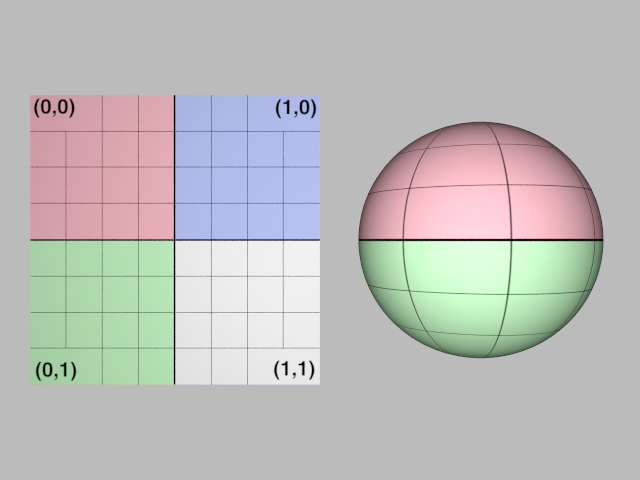
\includegraphics[width=0.19\linewidth]{imgs/hw_3_1a.png}
    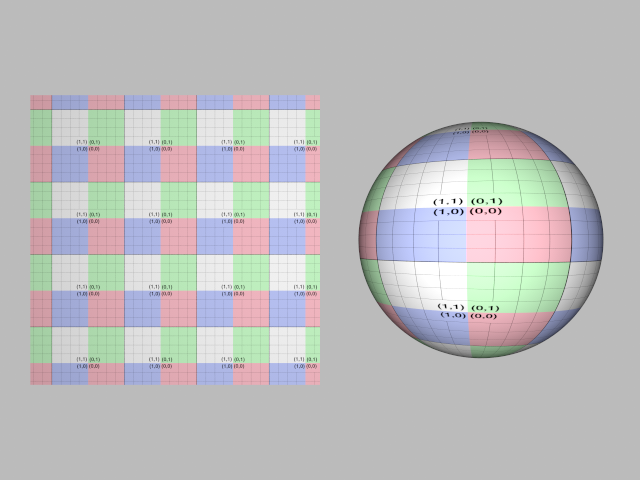
\includegraphics[width=0.19\linewidth]{imgs/hw_3_1b.png}
    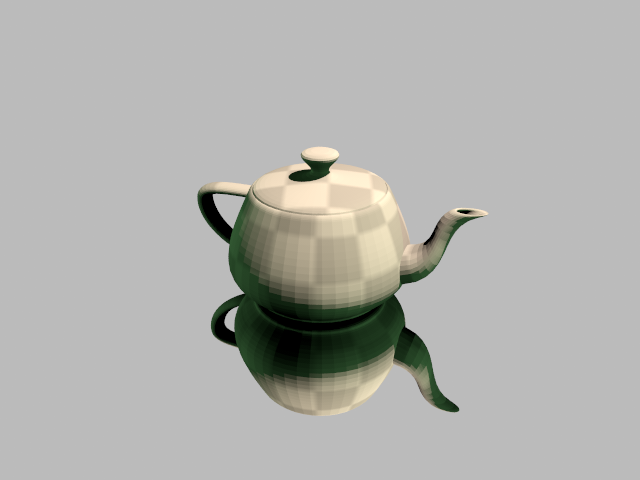
\includegraphics[width=0.19\linewidth]{imgs/hw_3_1c.png}
    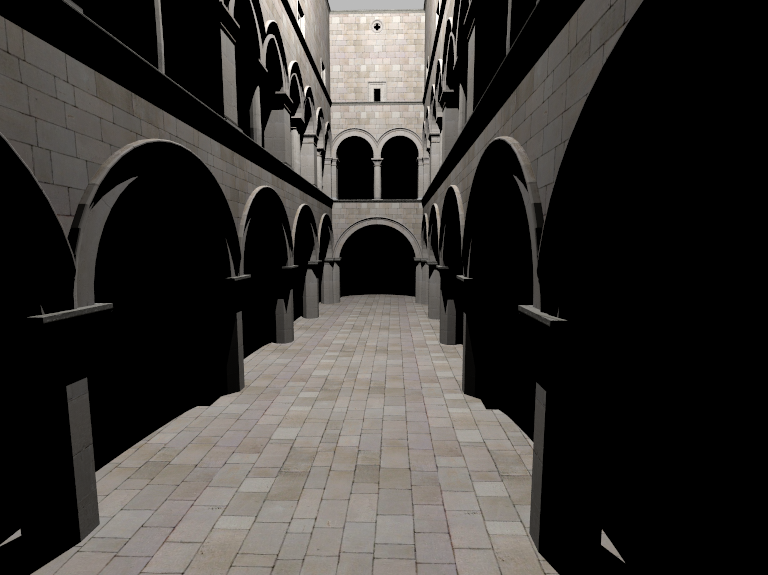
\includegraphics[width=0.19\linewidth]{imgs/hw_3_1d.png}
    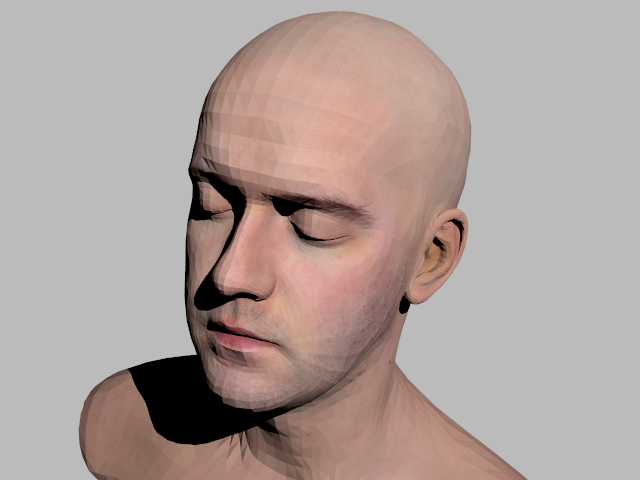
\includegraphics[width=0.19\linewidth]{imgs/hw_3_1e.png}
    \caption{Reference images for Homework 3.1.}
    \label{fig:hw_3_1}
\end{figure}

\section{Shading normals}
You have probably noticed that some of the 3D models we rendered look ``polygonal'', while we ideally want them to be smooth. One way to improve this is to increase the polygon count, but this approach seems expensive. \href{https://en.wikipedia.org/wiki/Phong_shading}{Phong} has come up with a genius way to make polygonal surfaces look smooth. The idea is to define a \emph{shading normal} per triangle vertex, and interpolate the normal within the triangle to have smooth normals. We will implement shading normals in this part.

Our \lstinline{ParsedTriangleMesh} can come with a field \lstinline{normals} which is its shading normals defined per-vertex (if \lstinline{ParsedTriangleMesh::normals.size() == 0}, then the mesh does not have shading normals). Once you hit a triangle, if it has a shading normal, interpolate the normals using the barycentric coordinates (just like how you interpolate the UV coordinates, but remember to \lstinline{normalize} after interpolation). Then, during shading, replace the normal you used with the interpolated shading normal.

As usual, type the following in the terminal to see your results:
\begin{lstlisting}[language=C++]
./torrey -hw 3_2 ../scenes/teapot/teapot_textured.xml
./torrey -hw 3_2 ../scenes/head/head.xml
\end{lstlisting}
You should render images like the ones in Figure~\ref{fig:hw_3_2}.

\begin{figure}[ht]
    \centering
    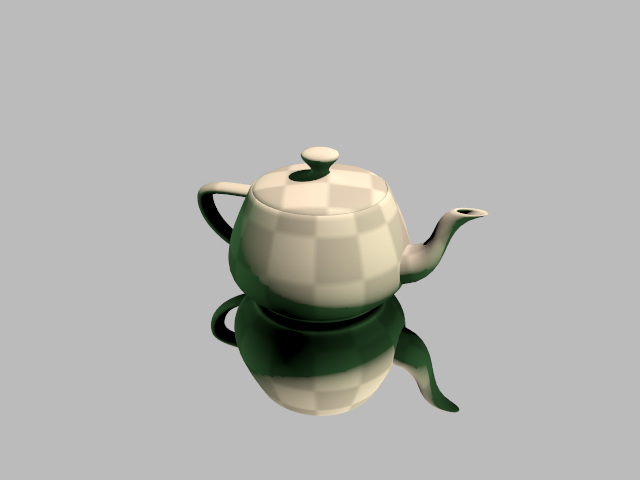
\includegraphics[width=0.3\linewidth]{imgs/hw_3_2a.png}
    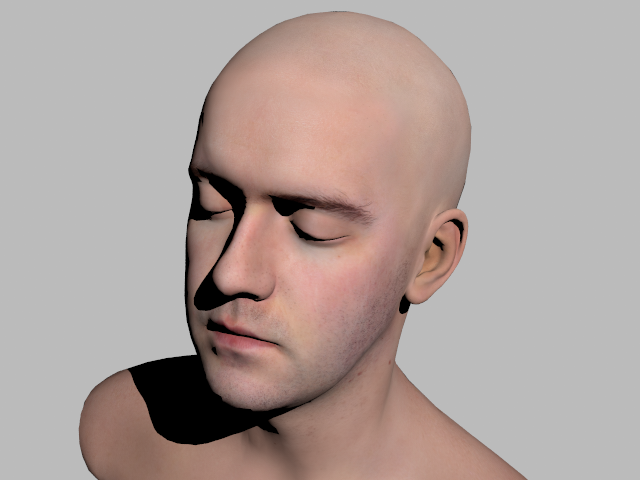
\includegraphics[width=0.3\linewidth]{imgs/hw_3_2b.png}
    \caption{Reference images for Homework 3.2.}
    \label{fig:hw_3_2}
\end{figure}

\paragraph{Quiz:} Why is the shadow boundary for the teapot still looks jaggy? Propose a way to fix it. (Hint: you may want to read Hanika's article on \href{https://jo.dreggn.org/home/2021_terminator.pdf}{Hacking the shadow terminator}.)

\section{BRDFs}
The materials we have currently are simplistic: real world materials spend a large spectrum between purely diffuse and purely specular. Let's implement a few more of them.

\subsection{Fresnel reflection}
Real world metals and mirrors do not reflect light equally at all angles. A prominent effect is predicted by French physicst \href{https://en.wikipedia.org/wiki/Augustin-Jean_Fresnel}{Fresnel} using the wave theory of light. For example, metals become more white when you look at it from a \emph{grazing angle}. Many materials also get more mirror-like when we look at them from grazing angles.

In graphics, we use an approximation proposed by \href{https://en.wikipedia.org/wiki/Schlick%27s_approximation}{Christophe Schlick}:
\begin{equation}
F = F_0 + (1 - F_0) \left(1 - n \cdot l\right)^5,
\label{eq:fresnel}
\end{equation}
where $n$ is the normal and $l$ is the unit direction towards the light source. $F_0$ is the reflection when light comes in perpendicularly to the surface. For glasses and dielectric materials, $F_0$ can be well approximated by the index of refraction ($F_0 = \left(\frac{\eta_i - \eta_o}{\eta_i + \eta_o}\right)^2$ where $\eta_i$ and $\eta_o$ are the index of refraction of the two sides of the surfaces). For metals or \emph{conductors}, the actual Fresnel equation requires the index of refraction number to be described using complex numbers, and the index of refraction differs a lot depends on the wavelength of light.\footnote{\href{https://www.feynmanlectures.caltech.edu/I_31.html}{Feynman's lectures of physics} has some good introduction to this, but you might need to start reading from earlier chapters to understand the chapter I linked.} Manipulating the complex number index of refraction is not intuitive, and we do not have textured data for them either. Therefore, a common solution that gives intuitive control to metal Fresnel is to directly specify $F_0$ in RGB.\footnote{I highly recommend watching \href{https://www.youtube.com/watch?v=kEcDbl7eS0w}{Natty Hoffman's presentation} on the topic of Fresnel equation.}

Let's first add the Fresnel term to our \lstinline{mirror} material. Instead of directly multiplying the color with the reflectance, we multiply it with the Schlick Fresnel (Equation~\eqref{eq:fresnel}). 

Let's use a scene from Homework 1 to test your result:
\begin{lstlisting}[language=bash]
./torrey -hw 3_3 ../scenes/hw1_spheres/scene1.xml
\end{lstlisting}

You should see something like Figure~\ref{fig:hw_3_3_fresnel}.

\begin{figure}[ht]
    \centering
    \includegraphics[width=0.4\linewidth]{imgs/hw_3_3a.png}
    \caption{Adding Fresnel reflection to the mirror spheres.}
    \label{fig:hw_3_3_fresnel}
\end{figure}

\paragraph{Quiz:} Change the direction $l$ to point towards the incoming ray direction in your code -- does it make a difference? Why?

Another good use of Fresnel equation is to blend between diffuse and specular materials. The physics work like this: many materials have multiple \emph{layers}. Many materials can be modeled using two layers: a dieletric \emph{coating} on top of a diffuse layer. For example, plastic, woods, and car paint usually are like this: they have an overall diffusive appearance, but also have the shiny smooth coating on top of the surface. When a light hits the dielectric layer, $F$ amount of light will reflect, and $1 - F$ amount of light will \emph{refract} into the diffuse layer. Thus we can often blend diffuse and specular layers using the Fresnel equation:
\begin{equation}
\text{specular} + (1 - F) \text{diffuse},
\end{equation}
where the specular term already includes the Fresnel equation. Figure~\ref{fig:real_world_fresnel} shows a real photograph demonstrating this effect: when we look at the table from the grazing angle, it becomes more specular, and when we look at the table from the top, it becomes more diffusive.
\begin{figure}[ht]
    \centering
    \includegraphics[width=0.3\linewidth]{imgs/fresnel_1.jpeg}
    \includegraphics[width=0.3\linewidth]{imgs/fresnel_2.jpeg}
    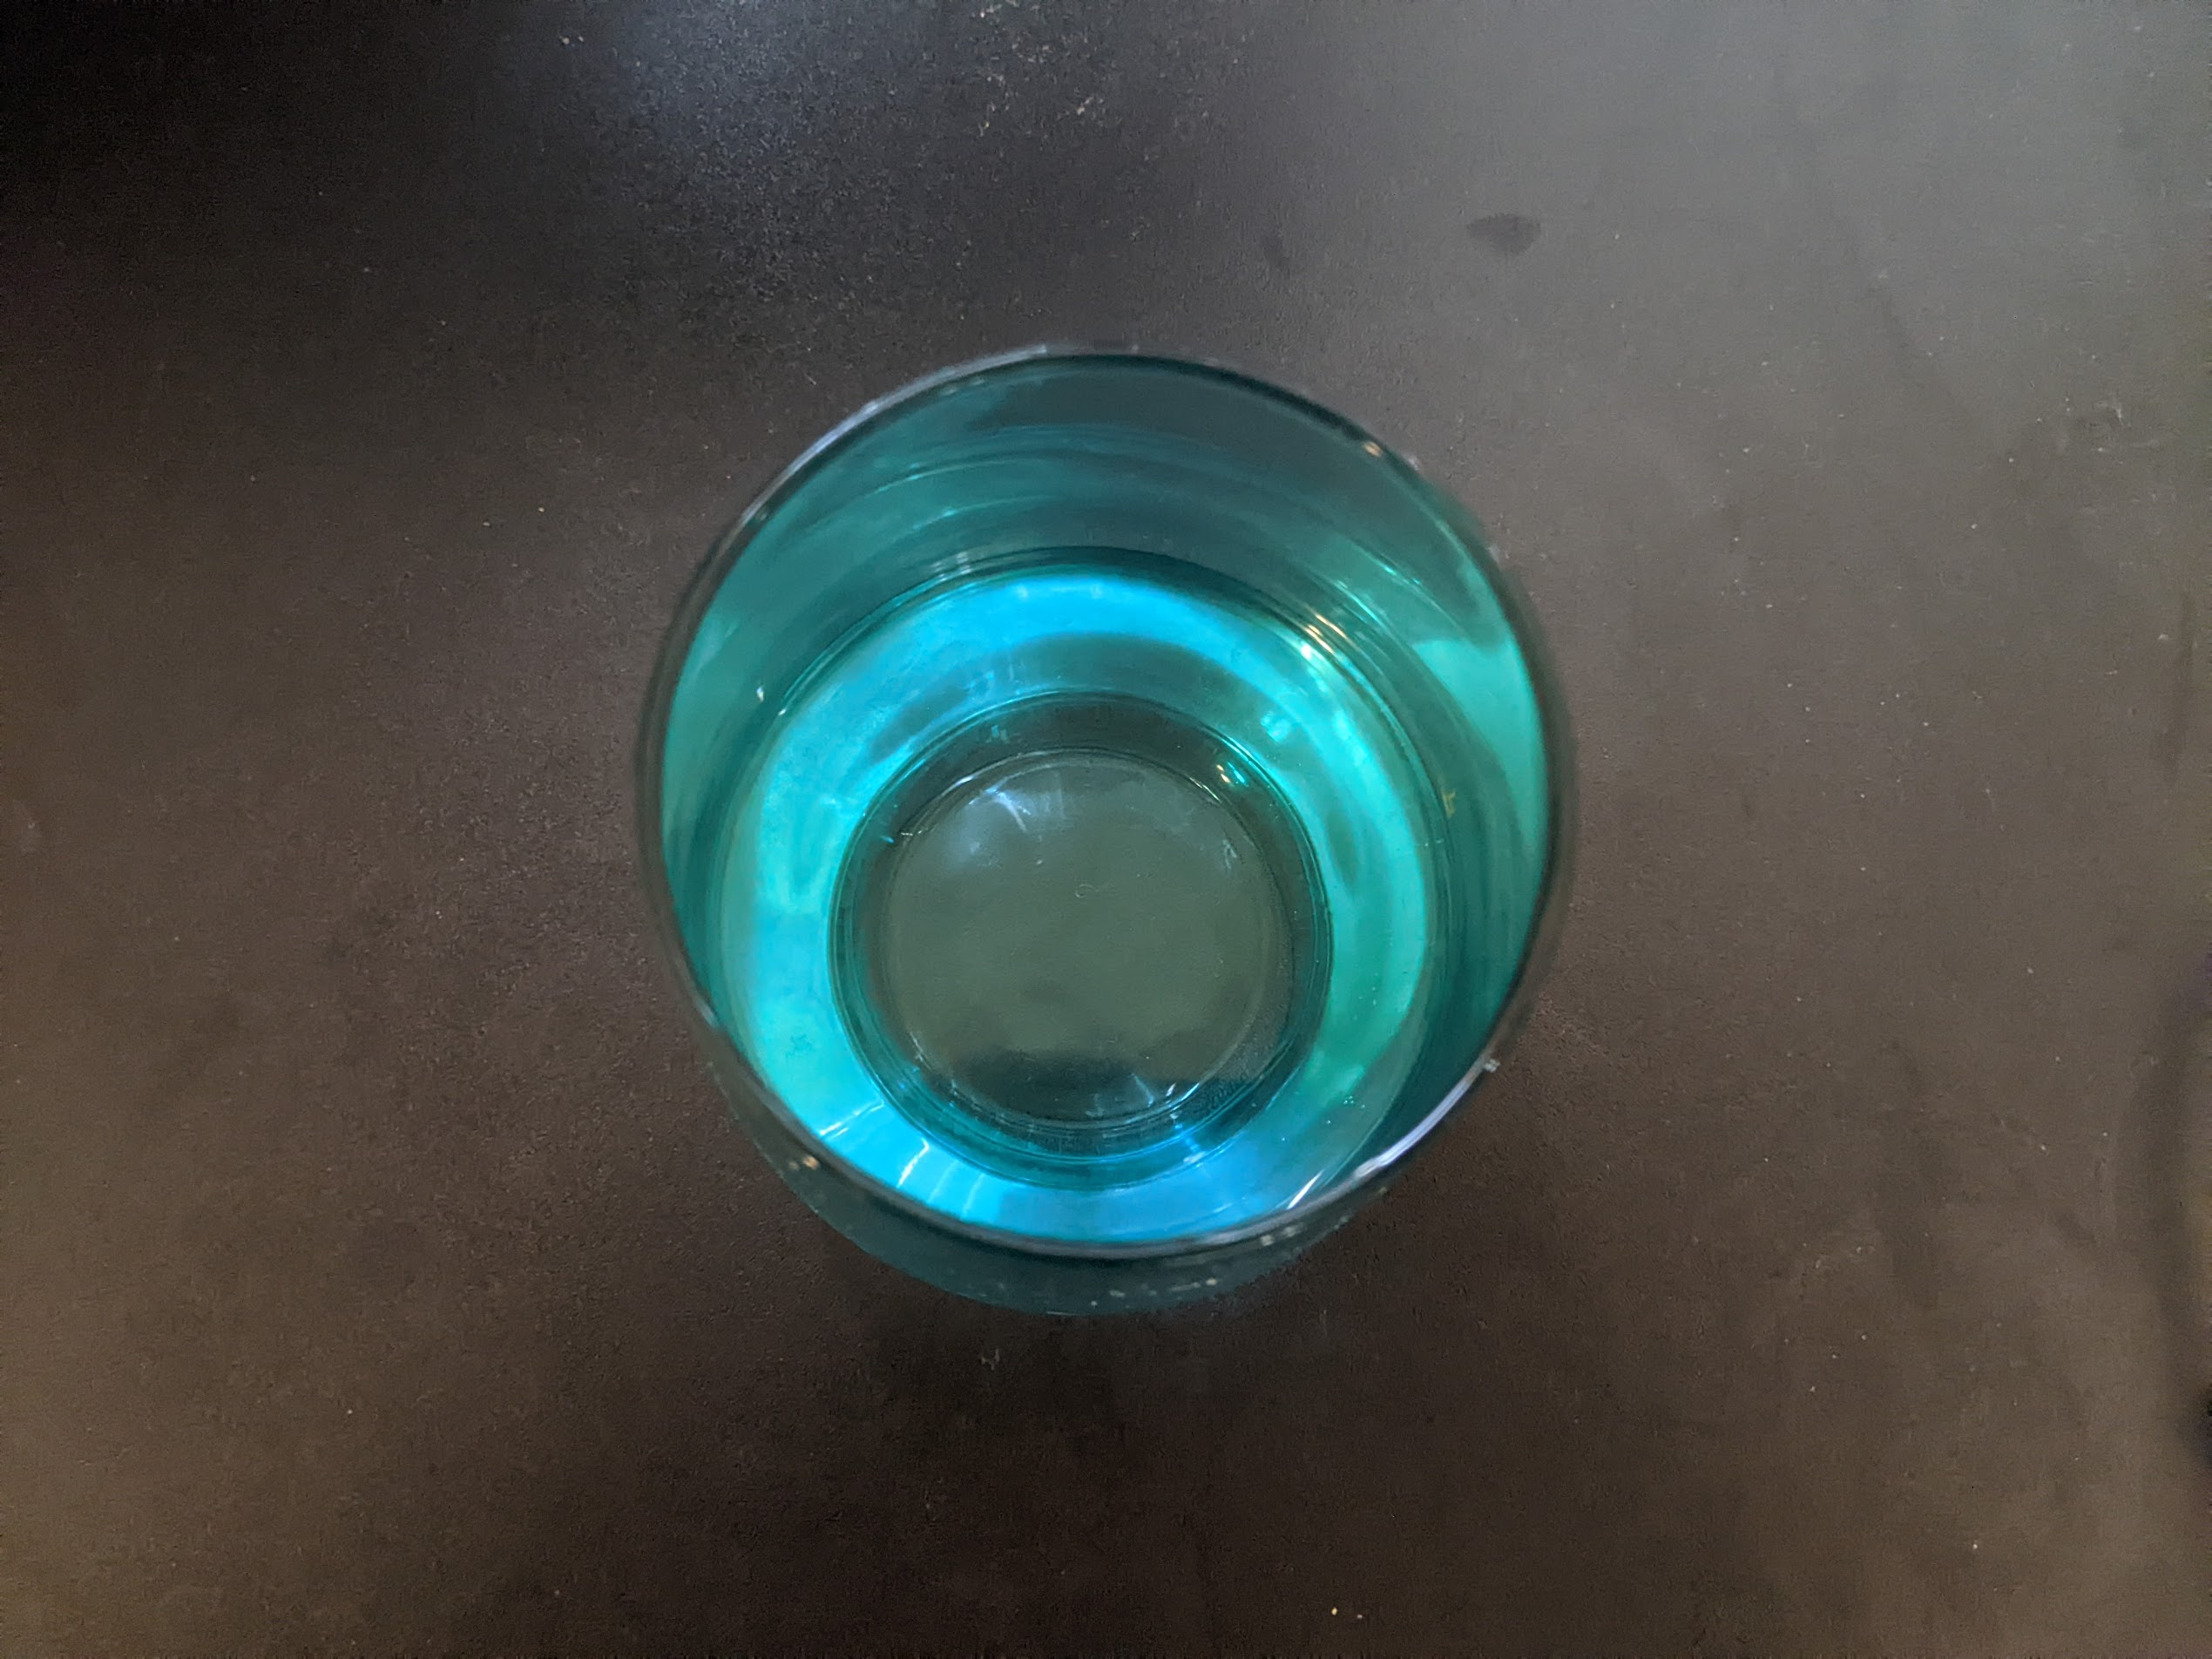
\includegraphics[width=0.3\linewidth]{imgs/fresnel_3.jpeg}
    \caption{Real world pictures showing the effect of Fresnel reflection on coated materials (look at the table).}
    \label{fig:real_world_fresnel}
\end{figure}
Since in this situation, the specular layer is usually dieletric, and these dielectric materials are usually monochromatic (i.e., the index of refraction is the same for all visible wavelength), we will use a single index of refraction parameter to control $F_0$. Assuming the index of refraction of air is $1$, we set $F_0 = \frac{\eta - 1}{\eta + 1}$ for all RGB. A common choice of $\eta$ is $1.5$.

Implement this Fresnel-based blending in the \lstinline{plastic} material (the information is stored in \lstinline{ParsedPlastic} in the scene).

\section{Area lights}
So far all our scenes are rendered with point lights. Point lights are nice for situations where you want your shadow to have hard boundaries, but sometimes we want softer lighting. We achieve this by turning our geometric objects themselves into lights. You can think of them as an infinite collection of small point lights (but each of them only emit light towards the direction the surface is facing, instead of emitting light to all directions).



%\bibliographystyle{plain}
%\bibliography{refs}

\end{document}
